\documentclass[11pt]{beamer}
\usetheme{default}

\usepackage[utf8]{inputenc}
\usepackage[T1]{fontenc}
\usepackage{amsmath}
\usepackage{amsfonts}
\usepackage{amssymb}
\usepackage{graphicx}

\author{Gregor Corbin}
\title{How to actually perform experiments in experimental mathematics}
\subtitle{For lazy people, a.k.a. mathematicians}
\logo{}
\institute{}
\date{}
\subject{}
\setbeamercovered{transparent}
\setbeamertemplate{navigation symbols}{}

\begin{document}
	\maketitle
	
	\begin{frame}{What is experimental mathematics?}
	
	\end{frame}
	
	\begin{frame}{What is an experiment?}
		content...
	\end{frame}
	
	\begin{frame}{How I performed 'experiments' previously}
		this is very \textbf{tedious}
	\end{frame}
	
	\begin{frame}{Achieving repeatability}
		Necessary information:
		\begin{itemize}
			\item the program source code
			\item all parameters (ini files, command line options)
			\item all data (mesh files, geometry data, ...)
			\item state of the environment (library/package versions, operating system, hardware, ...)
			\item the output / results 
		\end{itemize}

		Tasks: 
		\begin{itemize}
			\item When performing an experiment, log all this data
			\item When repeating an experiment, restore the complete state
		\end{itemize}
	\end{frame}
	
	\begin{frame}
		{
			\renewcommand{\arraystretch}{1.2}
			\begin{table}
				\begin{tabular}{l@{\hspace{5pt}}lr@{.\hspace{0pt}}l@{$\times$\hspace{0pt}}lcl}
					\multicolumn{2}{l}{Parameter}   &\multicolumn{3}{l}{Value}&                  & Description \\
					\hline 
					T           && $1$&$5768$&  $10^{ 7}$  & $s$              & time span = half a year \\
					c           && $2$&$1$   &  $10^{-4}$  & $ \frac{mm}{s}$  & cell speed \\
					$\lambda_0$ && $1$&$0$   &  $10^{-5}$  & $\frac{1}{s}$    & cell-state independent part of turning rate\\
					$\lambda_1$ && $2$&$5$   &  $10^{-4}$  & $\frac{1}{s}$    & cell-state dependent part of turning rate\\
					$k^+$       && $1$&$0$   &  $10^{-5}$  & $\frac{1}{s} $   & attachment rate of cells to ECM\\
					$k^-$       && $1$&$0$   &  $10^{-5}$  & $\frac{1}{s} $   & detachment rate of cells to ECM\\	
					%Number      &\multicolumn{3}{l}{Value}&                  & Interpretation \\
					\hline		
					$\epsilon$&$=St$&$3$&$02$  &  $10^{-1}$  &                  & Strouhal number\\
					$Kn         $&&$6$&$34$  &  $10^{-3}$  &                  & Knudsen number\\
					$R$&$= \frac{St^2}{Kn}$&$1$&$44$  &  $10^{1}$  &                  & \\
					$\eta$&$= \frac{\lambda_1}{\lambda_0}$&$2$&$5$& $10^{1}$  && Ratio of turning rate coefficients\\ 
				\end{tabular}
				\caption{The parameters and the resulting characteristic numbers used in the 2D brain slice simulation.}
				\label{tab:parameters}
			\end{table}
		}
	\end{frame}
	
	\begin{frame}{An example from a biology lab}	
		Tedious! Nobody here would ever do this.
	\end{frame}
	
	\begin{frame}{The good news}
		\begin{itemize}
			\item everything is run on a computer
			\item computers excel at automated,tedious tasks
		\end{itemize}
		Ideally all the logging and setup is done at the press of a single 'button'
		\begin{center}
			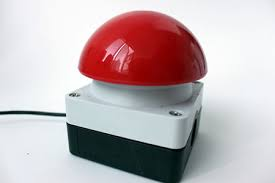
\includegraphics[height=0.3\textheight]{figures/redbutton}
		\end{center}
	\end{frame}
	
	\begin{frame}{Introducing the experiment suite}
		\framesubtitle{a.k.a. the button}
		content...
	\end{frame}
	
	\begin{frame}{Discussion}
		content...
	\end{frame}
			
\end{document}